\chapter{Mathematical Models and Theories}
In order to calculate the position of an object in a 3D space, from the use of 2D images from viewpoints, a number of steps are executed. Firstly it is necessary to calculate the angles from each viewpoint's centre to the object's position. The angle information from two or more viewpoints can then be combined to calculate the object's position in the global coordinate system defined in \cref{sec:coor} which makes the laser unit able to target it. The chapter presents how a pixel found in a image can be used to calculate the direction towards to target relatively from the given camera.

This chapter also presents the model for a \acrlong{pid} and how it is used when using DC motors. 

\section{Getting a Pixel's Offset}\label{ssc:xy_angles}
In \cref{ch:obj_rec} a basis for object recognition was presented which is used to identify a target that the system are tracking. Using object recognition the pixel which is the center of the target can be obtained. This pixel's position in an image is used to calculate the difference between the direction of a vector with base in the lens' centre and direction of the object. Figure \ref{fig:calculating_angles} illustrates an image where a pixel is used as identifier of the object. Two coordinate systems are defined on the image in order to obtain this direction, the first system has the axes $Offset_x$ and $Offset_y$ which are used to tell a pixel's position ont he image. The other coordinate system's origin is in the centre of the image and is used to define a vector with the tail placed in the camera's lens' centre. This vector is adjusted to point towards the intended object.

\begin{figure}[ht]
    \centering
    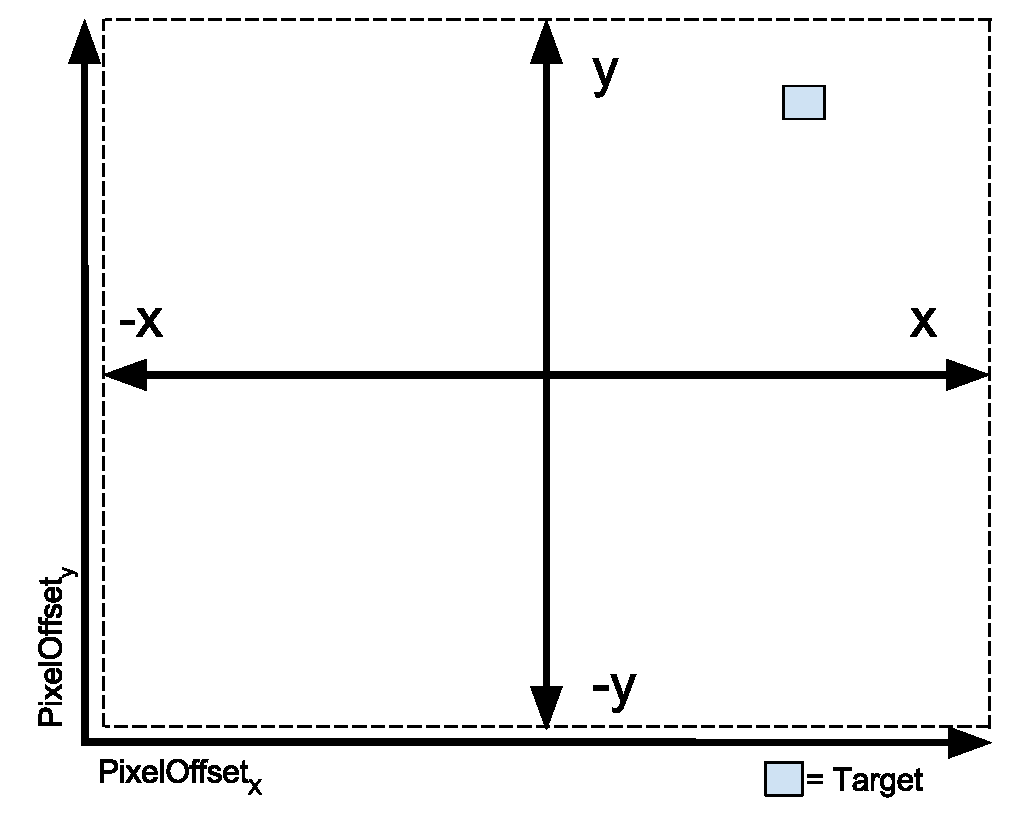
\includegraphics[scale=0.65]{graphics/signed_angles_simple.eps}
    \caption{Example with a marked centre and a target in top right quadrant}
    \label{fig:calculating_angles}
\end{figure}

Using the definition of the x- and y-axis from the image, the z-axis in the 3D room will also have origin in the centre of the lens, but the depth of the image will follow the negative z-axis, resulting in the vector, with tail in the lens, to be defined as
$\left[\!\begin{array}{c}
0\\
0\\
-1
\end{array}\!\right] $
since the vector's direction is away from the lens along the negative z-axis. Before adjusting this vector the deviation along the y- and x-axis must be found. The deviation is found by calculating the fraction of how much the object's pixel is along the two axes. The equations for this are:
\begin{equation}
\frac{Offset_X - 0.5 * Width}{0.5 * Width} \label{eq:offset-x}
\end{equation}
\begin{equation}
\frac{Offset_Y - 0.5 * Height}{0.5 * Height} \label{eq:offset-y}
\end{equation}
\Cref{eq:offset-x} and \cref{eq:offset-y} show the fraction of how far the pixel is along the x- and y-axis, respectively. With the knowledge of these offsets it is possible to calculate the angles for which the vector shall be rotated. A camera has one \acrfull{fov} for each axis. The angles of these \glspl{fov} are used to calculate how many degrees the pixel has moved along the axes. The \gls{fov} is included in \cref{eq:offset-x_fov} and \cref{eq:offset-y_fov}, as $F_x$ for the horizontal \gls{fov} and $F_y$ for the vertical \gls{fov}. Furthermore, the \gls{fov} is halved because the angles are found relative to the centre.

\begin{equation}
\frac{Offset_X - 0.5 * Width}{0.5 * Width}*F_x*0.5 \label{eq:offset-x_fov}
\end{equation}
\begin{align}
\frac{Offset_Y - 0.5 * Height}{0.5 * Height}*F_y*0.5 \label{eq:offset-y_fov}
\end{align}

\Cref{eq:offset-x_fov} and \cref{eq:offset-y_fov} are the final equations that are used for the calculations of the angles. The following section will focus on the rotation of matrices around the x- and y-axes. Lastly an example is given to illustrate the use of the techniques.
\section{Calculating Rotations}
\Cref{ssc:xy_angles} defined how a 2D image is analysed to find the difference, in degrees, between a centred vector and the location of an object. The following section explains how this centred vector is rotated to intersect the targeted object in 3D space.

The angles are found on the x- and y-axis meaning the rotations will be performed on these axes. The rotation matrices needed are shown in \cref{eq:rotation_x} and \cref{eq:rotation_y} respectively.


\begin{equation}\label{eq:rotation_x}
\begin{bmatrix}
1 & 0 & 0 \\
0 & cos\theta & -sin\theta \\
0 & sin\theta & cos\theta \\
\end{bmatrix}
\end{equation}

\begin{equation}\label{eq:rotation_y}
\begin{bmatrix}
cos\theta  & 0 & sin\theta \\
0 & 1 & 0 \\
-sin\theta & 0 & cos\theta \\
\end{bmatrix}
\end{equation}

The rotation matrices rotate vectors counter clockwise from their original direction. \Cref{fig:signed_angles} shows how these rotations are represented in the images.
\begin{figure}[H]
    \centering
    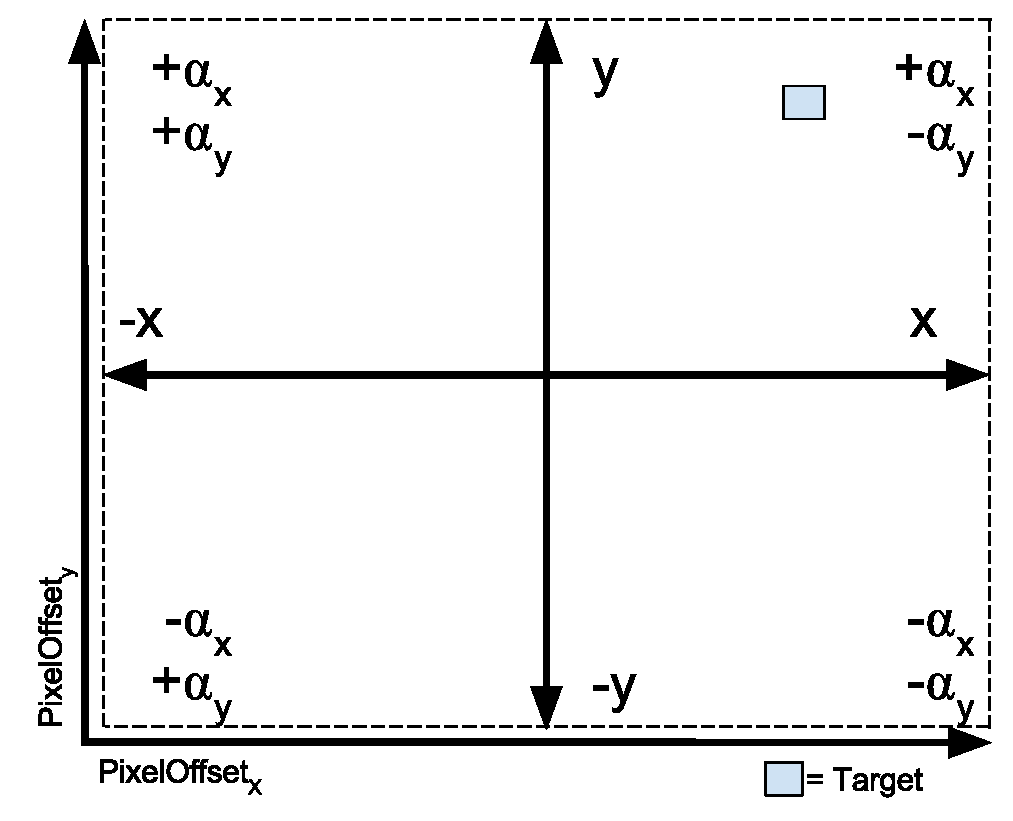
\includegraphics[scale=.65]{graphics/signed_angles.eps}
    \caption{Example showing angle values, depending on graph quadrants}
    \label{fig:signed_angles}
\end{figure}

Looking at the first quadrant containing the target, the rotation around the x-axis must be a counter clockwise rotation from center origin, which is why the degrees must be positive. \Cref{eq:offset-y_fov} returns positive values when target is greater than half the height of the image, therefore, this equation returns the wanted result. \Cref{eq:offset-x_fov} however, returns negative values when target is on the left side of the image and positive values when the target is on the right side of the image, which is opposite from the wanted behaviour. This behaviour is easily achieved however, by negating the result of \cref{eq:offset-x_fov}, resulting in \cref{eq:offset-x_opt}
\begin{align}
-\left(\frac{Offset_X - 0.5 * Width}{0.5 * Width}\right)*F_x*0.5
\label{eq:offset-x_opt}
\end{align}
The following section gives an example of finding the angle derivations and then rotating the lens' centre vector to cut the target's position.

\section{Example of Calculations}
A picture is taken with a camera and an object is defined to be located at the first quadrant of the image, with a pixel offset of $(x,y)=(500,400)$, the size of the image is $640x480$ $pixels$ and the \gls{fov} of the camera is $62\degree$. This information is inserted into \cref{eq:offset-y_fov} and \cref{eq:offset-x_opt}, giving:
\begin{align}
-\left(\frac{500 - 0.5 * 640}{0.5 * 640}*F_x*0.5\right) = -17.44\degree
\label{eq:ex_offset-x_opt}
\end{align}
\begin{align}
\frac{400 - 0.5 * 480}{0.5 * 480}*F_y*0.5 = 20.67\degree
\label{eq:ex_offset-y}
\end{align}

Next is to rotate the wanted vector which is the camera lens' vector previously defined as
$\left[\!\begin{array}{c}
0\\
0\\
-1
\end{array}\!\right] $
 it has to be rotated $20.67\degree$ around the x-axis and $-17.44\degree$ around the y-axis. which is shown in \cref{eq:rotation_on_x_and_y_part1} and \cref{eq:rotation_on_x_and_y_part2}.
\begin{equation}\label{eq:rotation_on_x_and_y_part1}
\begin{bmatrix}
1 & 0 & 0 \\
0 & cos(20.67) & -sin(20.67) \\
0 & sin(20.67) & cos(20.67)
\end{bmatrix}
\begin{bmatrix}
0 \\
0 \\
-1
\end{bmatrix}
=
 \begin{bmatrix}
0 \\
0.353\\
-0.936
\end{bmatrix}
\end{equation}
\begin{equation}\label{eq:rotation_on_x_and_y_part2}
\begin{bmatrix}
cos(-17.44)  & 0 & sin(-17.44) \\
0 & 1 & 0 \\
-sin(-17.44) & 0 & cos(-17.44)
\end{bmatrix}
\begin{bmatrix}
0 \\
0.353\\
-0.936
\end{bmatrix}
=
 \begin{bmatrix}
0.280 \\
0.353 \\
-0.893
\end{bmatrix}
\end{equation}
$\left[\!\begin{array}{c}
0.280 \\
0.353 \\
-0.893
\end{array}\!\right] $
is the vector in the local coordinate system of the camera, which cuts the object. This vector has to be transmuted into the global coordinate, so the actual position of the object can be calculated for the 3D space.

\section{\acrlong{pid} Controller}
\label{ss:pid}
The motors used with the \gls{nxt} are assumed to be cheap in the sense there is no guarantee that an instruction is carried out as precisely as specified. For example, it cannot be assumed that two of the same motors will yield an identical result when instructed to run for a given time frame. The motors are \glspl{dcm}, so it is not possible to instruct them to turn a certain amount of degrees.
To regulate and make sure the motors controlling the targeting device are responsive, as well as carry out the instructions given as precise as possible, it has been chosen to use a \gls{pid} controller. This controller is essentially an algorithm which takes feedback into consideration and compensates for it. It regulates the power at which the motor is working, increasing the power when the motor is far away from its target, and decreasing the power as it approaches the desired angle.  
The mathematical formula for this controller is as follows \citep{pid_controller}:

\begin{equation} \label{pid_formula}
[PID-controller] \
u(t) = K_p *e(t) + K_i \int_0^t e(\tau)d\tau + K_d*
\frac{de}
     {dt}
\end{equation}
There are several adjustable constants denoted by $K$. The algorithm consists of three terms. The first term, $K_p*e(t)$ is a constant multiplied by a tracking error, which is the running difference between the desired input value and the current actual value. The second term, $K_i \int_0^t e(\tau)d\tau$, is a constant multiplied by the running summation of errors. The third term, $K_d* \frac{de}{dt}$, is the last constant multiplied by the difference between the current error and the previous error from last iteration. $dt$ is the interval at which the function is executed in milliseconds, and can be integrated into the three adjustable constants when the controller has a well-defined, confined purpose.

The adjustable parameters all have a specific influence on the controller, as can be seen in table \ref{pid_char}. There are four factors that to some extent are influenced by each of the parameters. Rise time is the time it takes to reach the desired value. Overshoot encodes the degrees of overshoot on the first rise. Settling time is the time it takes to settle itself within a certain range of the desired value. S-S error is short for steady-state error, and is responsible for the difference between the actual final value and the desired value.
These factors are illustrated on the graph shown on \ref{fig:pid_graph} with example values for the parameters.
\begin{table}[H]
\begin{tabular}{|l|l|l|l|l|}
\hline
RESPONSE & RISE TIME    & OVERSHOOT & SETTLING TIME & S-S ERROR \\ \hline
Kp          & Decrease     & Increase  & Small Decrease  & Decrease  \\ \hline
Ki          & Decrease     & Increase  & Increase      & Eliminate \\ \hline
Kd          & Small Increase & Decrease  & Decrease      & No Change \\ \hline
\end{tabular}
\caption{Table showing parameter influence based on \citep[University of Michigan]{pid_controller}}
\label{pid_char}
\end{table}

\begin{figure}[H]
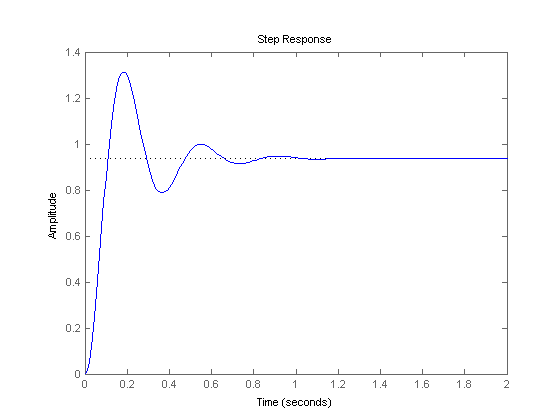
\includegraphics[scale=1]{graphics/pid_graph.png}
\caption{Example graph of a \gls{pid} controllers effect over time with example constant values\cite{pid_controlle_picr}}
\label{fig:pid_graph}
\end{figure}
Using the graph seen on \ref{fig:pid_graph} as an example, the rise time is approximately 0.1 sec, overshoot is 0.3 amplitude, settling time is around 1 second with very little error, and the steady-state error is approximately 0 amplitude. The constants can be fine-tuned to reduce and eliminate these factors.

To be able to adapt the \gls{pid} controller to the \gls{nxt} motors it will be necessary to customize different values for the two motors, as they operate under different loads. The three parameter values are easily found from similar projects, however the different weights on the motors cause this to be a unique case, which incites an alteration. The minimum power for the two motors to operate is different because of the load differences, as explained in \cref{sc:rig}. If this is not taken into account, the controller will never be able to reach its desired value, as it will get close enough for the power value to be beneath the threshold of what the motor needs to operate. Because of this it will be necessary to analyse the output and correct for this case.

\subsection{Termination}
To use a \gls{pid} in a system with real-time requirements it is necessary to impose restrictions on the run-time of the controller. Furthermore, it has to be constructed in such a way that it is possible to determine when the controller has succeeded, meaning the motors are at the desired angles, and the controller is ready for new input. This check can be done by monitoring certain values of the controller; specifically the derivative, which is calculated by finding the difference between the current error and the previous error. It can be assumed that the \gls{pid} has succeeded once the derivative has been equal to zero over a predefined period of time. To strengthen this assumption there can also be checks on the current position of the motors and on the speed of the motor.

A challenge the controller faces is being in charge of two motors instead of one. It is desired that both motors are moving at the same time, as running them in sequence significantly increases the time spent by the controller. Early in the process it became clear that problems arose from two motors running simultaneously. When one motor has finished before the other, the second motor's movement can cause vibrations resulting in the first motor moving a degree away from target. To fix this, a check is added once both motors have finished their movement, confirming the final position is on target. If this is not correct, the controller will iterate over itself once again to fix this error.

The run-time restrictions imposed on the \gls{pid} manifest themselves by a limit on the iterations of the function. After a constant amount of iterations, the controller will be forced to finish even if the target has not been reached. When calculating this amount, the speed of the processor has to be taken into consideration, as a fast processor might be capable of going through all iterations faster than the time it takes for the physical movement. This opens up for the possibility of making worst-case complexity analysis of the controller and schedule it.
